\documentclass{article}
\usepackage{graphicx}
\usepackage{lipsum}
\usepackage{tocloft}
\usepackage{float}
\usepackage{subcaption}
\usepackage{hyperref}
\usepackage[nottoc]{tocbibind}
\usepackage{threeparttable}
\usepackage{attachfile2}
\usepackage{amsmath}
\usepackage{booktabs}



\setcounter{tocdepth}{3}

\setlength{\parindent}{0pt}

\title{Pricing and Credit Risk Implications of GSE Privatization: A Fixed Income Perspective}
\author{}
\date{}

\begin{document}

\maketitle

\tableofcontents
\vspace{1em}
\noindent Word Count: 1838

\newpage

\section{Executive Summary}


\section{Part I: Bond Pricing and Interest Rate Risk}
\subsection{Objective}
The objective of Part I is to evaluate the pricing and interest rate sensitivity of three fixed income securities: one non-callable and two callable bonds.

\subsection{Assumptions and Setup}

We employed the continuous-time Vasicek model framework to price bonds, calibrated based on historical one-year U.S. Treasury yields\footnote{Converted the date strings to a datetime index and then resampled from quarterly to annual frequency, taking each year’s first observation.} (DGS1 series) from 2004 to 2024. \\

During calibration, we performed a first-order autoregression (AR(1)) on the DGS1 time series data to estimate the following Vasicek parameters: the long-term mean interest rate ($\theta$), the speed of mean reversion ($\kappa$), and the volatility ($\sigma$). The starting short rate for the tree was set at 3.88\%, matching the observed one-year rate. \\

We assumed a risk-neutral environment and the market price of risk parameter $\lambda$ was set to 0. This assumption simplified the construction of the short-rate tree by allowing probabilities to be determined directly from the model without additional risk adjustments. We acknowledge this assumption may understate risk premia, but it allows a transparent, interpretable tree for callable valuation. \\

After parameter estimation, we constructed rate trees for each approach and priced bonds by backward induction, discounting cash flows according to the modeled short-rate paths. \\

For all three bonds, we assumed a face value of 100, a 3.5\% annual coupon, six-year maturity, and continuous compounding. When presented with the values of Delta in the tables, they were calculated using an infinitesimal change in rates. Furthermore, the values represent a 100bp change, i.e., a value of 5 would mean that a 1\% increase in rates leads to a 5 dollar decrease in bond price. \\


\begin{figure}[H]
    \centering
    \begin{subfigure}[b]{0.45\textwidth}
        \centering
        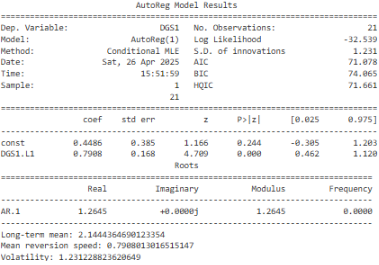
\includegraphics[width=\textwidth]{AR(1).png}
        \caption{AR(1) Regression Estimates}
        \label{fig:ar1}
    \end{subfigure}
    \hfill
    \begin{subfigure}[b]{0.45\textwidth}
        \centering
        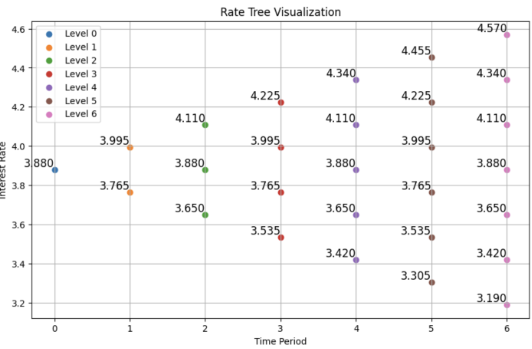
\includegraphics[width=\textwidth]{Screenshot 2025-04-26 233325.png}
        \caption{Binomial Tree}
        \label{fig:ar2}
    \end{subfigure}
    \caption{Calibrated Vasicek Model}
    \label{fig:comparison}
\end{figure}


\subsection{Bond 1: Non-Callable Coupon Bond}

\begin{figure}[H]
    \centering
    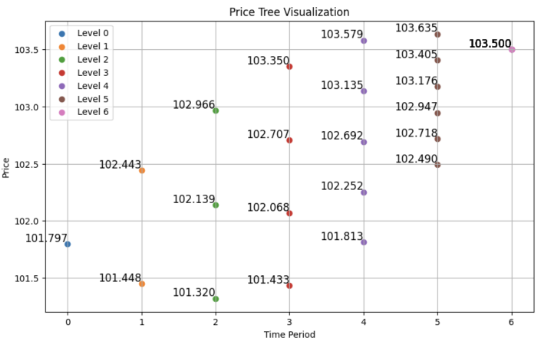
\includegraphics[width=0.5\linewidth]{Price Tree.png}
    \caption{Non-Callable Coupon Bond Price Tree}
    \label{fig:enter-label}
\end{figure}

We priced the non-callable coupon bond using three approaches, each incorporating different assumptions about interest rate dynamics. \\

\begin{table}[ht]
\centering
\begin{tabular}{l r r}
\hline
Approach                                  & Price (\$)  & Delta \\
\hline
Approach 1: STRIPS Curve          & 95.040    & 5.224 \\
Approach 2: SSE Calibration  & 95.350    & 4.273 \\
Approach 3: AR(1) Estimation      & 101.797   & 6.000 \\
\hline
\end{tabular}
\caption{Prices and Deltas of 6‐Year Non‐Callable Coupon Bonds}
\end{table}

\subsubsection{Approach 1: Strips Yield Curve Discounting}
The first method priced the bond by discounting each cash flow using the Strips yield curve. While straightforward, this approach does not account for interest rate volatility or mean reversion, and provides only a static valuation. As expected, the price under this method was higher than that of callable bonds, which are typically discounted for embedded option risk. \\

\subsubsection{Approach 2: Vasicek Model Calibrated to the Strips Curve}
The second method calibrated all parameters of a continuous-time Vasicek model to the Strips yield curve through SSE. This dynamic model better captures uncertainty in rates but risks overfitting to current market conditions, limiting its forecasting ability. This approach gives us a solution, but the parameters are not insightful, e.g. not very realistic values for phi and sigma because the objective function is quite flat and does not impose a lot of constraints on the problem. 

\subsubsection{Approach 3: Vasicek Model Based on Historical Treasury Data}
The third approach estimated Vasicek parameters, long-term mean ($\theta$), mean reversion speed ($\kappa$), and volatility ($\sigma$) through an AR(1) regression on historical one-year Treasury rates from 2004 to 2024. Using these parameters, we built a short-rate tree with an initial rate of 3.88\% and priced the bond via backward induction using probabilities. \\

This model produced a higher bond price compared to Approach 1, driven by a strong mean reversion effect ($\kappa = 0.79$) toward a low long-term mean (2.14\%). We assumed $\lambda = 0$, implying a risk-neutral setting where no compensation for interest rate risk is required—a simplification that facilitates tree construction but may underestimate true risk premia. \\

Moving forward with the pricing of the callable bonds, we will be using Approach 3 as it is the most informative and forward-looking. 

\subsection{Bond 2: European Callable Bond}

\begin{table}[ht]
\centering
\begin{tabular}{l r}
\hline
Quantity & Value \\
\hline
European Call Option Price (\$) & 0.3301 \\
European Callable Bond Price (\$) & 101.4669 \\
Delta of European Callable Bond ($ \Delta  $) & 5.792 \\
\hline
\end{tabular}
\caption{European Call Option and Callable Bond Valuation Results}
\end{table}


First, we build a bond price tree and a short rate tree over six years, aligning with the bond’s stated 6-year maturity. To correctly model risk-neutral valuation, we also construct a probability tree based on the Vasicek dynamics, where probabilities at each node are determined by the short rate’s drift and volatility; this is consistent with the assumption that rates follow a mean-reverting stochastic process. The non-callable bond price is taken as the starting node of the price tree, which reflects the expected discounted cash flows, consistent with no embedded options. \\

To value the call feature, we treat it as a European call option on the bond: at year 6, we calculate payoffs based on the excess of bond prices over the exercise price, assuming no early exercise, which is appropriate because the option is European style. We back-propagate these payoffs through the tree using risk-neutral expectations and discounting at the modeled short rates. The callable bond price is computed by subtracting the call option value from the non-callable bond value, under the standard assumption that the issuer owns the option and benefits from calling the bond. \\

To estimate delta, we approximate the sensitivity of the option value to small changes in the short rate using a central finite difference method, a standard and justified technique when analytical formulas are not available. Finally, we adjust the callable bond’s delta by subtracting the call option's delta from the non-callable bond's delta. Throughout, our approach ensures that the maturity structure, risk-neutral valuation, and treatment of the call feature are internally consistent and supported by the Vasicek modeling assumptions.


\subsection{Bond 3: American Callable Bond}

\begin{table}[ht]
\centering
\begin{tabular}{l r}
\hline
Quantity & Value \\
\hline
American Call Option Price (\$) & 0.0861 \\
American Callable Bond Price (\$) & 101.7109 \\
Delta of American Callable Bond ($ \Delta  $) & 5.596 \\
\hline
\end{tabular}
\caption{American Call Option and Callable Bond Valuation Results}
\end{table}


First, we use the same bond price tree, short rate tree, and probability tree built under the Vasicek model, ensuring consistency with the bond’s 6-year maturity and risk-neutral valuation framework. To value the American call feature, we construct an option value tree by setting the final payoffs at maturity (year 6) based on the maximum of the bond price minus the exercise price and zero. \\

Working backward through the tree, at each earlier node, we calculate the expected continuation value by taking the probability-weighted average of future option values, discounted appropriately using the short rate at that node. However, because this is an American-style option, we compare the immediate exercise value to the continuation value at each step and take the maximum. This captures the flexibility of the issuer to call the bond at any time up to maturity, consistent with the definition of an American option. \\

The American callable bond price is then computed by subtracting the American call option price from the non-callable bond price, under the standard assumption that the issuer owns the option and exercises it optimally for their benefit. To estimate delta, we approximate the sensitivity of the American call option value to small changes in the short rate using a central finite difference method, which is appropriate because closed-form derivatives for American options typically do not exist. \\

We then adjust the callable bond’s delta by subtracting the option's delta from the non-callable bond's delta. This ensures that the maturity structure, early exercise feature, and sensitivity calculations are internally consistent with the Vasicek assumptions and the American exercise behavior.


\section{Part II: Credit Risk Analysis}
\subsection{Objective}
The objective of Part II is to explain the nature of the default risk involved and identify the credit spread that would be incurred in the absence of government backing. 

\subsection{Data and Parameter Estimation}

To quantify Freddie Mac’s credit risk under a privatization scenario, we first assembled the necessary balance‐sheet and market inputs as of year‐end 2024.  Equity values \(E\) were taken from the company’s reported shares outstanding multiplied by the closing stock price.  Equity volatility \(\sigma_{E}\) was estimated iteratively until it converged.  Total debt \(F\) was obtained from the book value of all on- and off-balance sheet obligations reported in the 2024 10-K.  We set the risk-free rate \(r_{f}\) equal to the prevailing 10-year Treasury yield at the measurement date, and we chose a time to maturity \(T\) of ten years to match the typical remaining tenor of Freddie Mac’s liabilities. \\

Under the Merton framework, the firm’s asset value \(V\) and asset volatility \(\sigma_{V}\) are not directly observable.  We therefore back out \(\sigma_{V}\) by solving the single‐equation relationship
\[
  \sigma_{E}
  \;=\;\sigma_{V}\,V\,N(d_{1})
  \quad\text{where}\quad
  d_{1}
  =\frac{\ln\!\bigl(V/F_{\rm eff}\bigr)+(r_{f}+\tfrac12\sigma_{V}^{2})T}{\sigma_{V}\sqrt{T}},
\]
and \(F_{\rm eff}=F\,e^{-r_{f}T}\) is the present value of debt.  We fix
\[
  V \;=\;F_{\rm eff}\;+\;E
\]
with which we numerically solve for \(\sigma_{V}\). \\

We find these parameter estimates:

\begin{table}[H]
\centering
\begin{tabular}{@{}ll@{}}
\toprule
\textbf{Parameter} & \textbf{Estimate} \\
\midrule
Equity value, $E$ (trillions)            & 0.00337      \\
Equity volatility, $\sigma_E$            & 72\%         \\
Risk-free rate, $r_f$                    & 4.29\%       \\
Debt face value, $F$ (trillions)         & 3.305        \\
Time to maturity, $T$ (years)            & 10           \\
Implied asset value, $V$ (trillions)     & 1.997095     \\
Asset volatility, $\sigma_V$             & 1.6151\%     \\
\bottomrule
\end{tabular}
\caption{Parameter Estimates Used In The Merton Model Calibration}
\label{tab:parameter_estimates}
\end{table}


\subsection{Structural Approach: Merton Model}

With \(\sigma_{V}\) in hand, we proceed to compute the model‐implied credit spread:

\begin{enumerate}
  \item Compute 
  \[
    d_{2} \;=\; d_{1}\;-\;\sigma_{V}\,\sqrt{T}.
  \]
  \item Calculate the risk-neutral value of the firm’s debt:
  \[
    D \;=\;
      V\,N\bigl(-d_{1}\bigr)
    \;+\;
      F_{\rm eff}\,N\bigl(d_{2}\bigr),
  \]
  where \(N(\cdot)\) is the standard normal CDF.
  \item Back out the implied yield \(y\) by equating \(D\) to the discounted face:
  \[
    D \;=\; F\,e^{-yT}
    \quad\Longrightarrow\quad
    y \;=\; -\frac{1}{T}\ln\frac{D}{F}.
  \]
  \item Finally, report the credit spread in basis points:
  \[
    \text{Credit Spread}
    \;=\;
    \bigl(y - r_{f}\bigr)\times 10{,}000.
  \]
\end{enumerate}

We find the credit spread to be 0.7643\%.

\subsection{Part II: Discussion}
Our Merton model yields a stand-alone credit spread of 76 bp. Parrott \& Zandi note that, in a no-backstop scenario, rating agencies would resurrect their “stand-alone” ratings and place the GSEs well below their current Aaa/Aa status—historically around the mid-BBB range. Yet today’s market-observed non-callable Freddie spreads sit at only 15–30 bp, a direct reflection of the implicit government guarantee. The gap between our 76 bp model spread and the sub-30 bp market spread quantifies the value investors place on that backstop. \\

However, mapping 76 bp to actual corporate-bond indices suggests an even higher standalone rating than mid-BBB. On April 24, 2025 the ICE BofA AAA US Corporate Index OAS was just 43 bp, while the ICE BofA BBB US Corporate Index OAS was around 135 bp . Spreads on Single-A corporates typically trade in the 60–100 bp range, so our 76 bp implied spread aligns with an A-rated credit (e.g., S\&P A/A-2 or Moody’s A2/A3). In other words, stripping out the implicit guarantee would reprice Freddie Mac’s bonds toward the levels demanded by other large, highly rated financial issuers, rather than near-risk-free Treasuries.

\section{Limitations}

\begin{itemize}
    \item \textbf{Data Smoothing:} Annualized resampling of quarterly data may smooth over short-term volatility, potentially underestimating model volatility ($\sigma$).
\end{itemize}

\begin{itemize}
    \item \textbf{Risk-Neutral Assumption:} Setting the market price of risk parameter ($\lambda$) to zero simplifies tree construction but neglects liquidity premiums and credit spreads even present in Treasury markets.
\end{itemize}

\begin{itemize}
    \item \textbf{Discretization Error:} Using a binomial tree with six annual time steps introduces discretization error; finer time intervals would improve accuracy but increase computational complexity.
\end{itemize}

\begin{itemize}
    \item \textbf{Unobservable Inputs in Merton Model:} Calibrating the Merton model requires assumptions about firm asset value and volatility, which are not directly observable, making the model sensitive to estimation errors.
\end{itemize}

\begin{itemize}
    \item \textbf{Simplified Default Assumption:} The Merton model assumes default occurs only at maturity and solely due to asset value falling below debt, ignoring early default events and liquidity-driven failures.
\end{itemize}


\section{Appendix}

\begin{figure}[H]
    \centering
    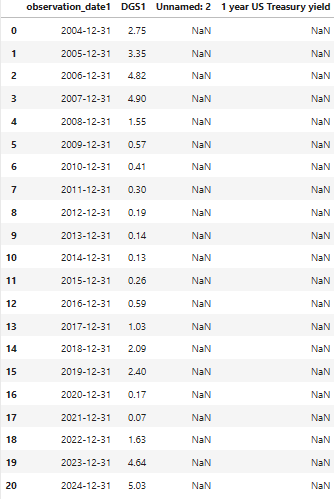
\includegraphics[width=0.5\linewidth]{Screenshot 2025-04-26 225705.png}
    \caption{DGS1 Quarterly Observations 20 Years}
    \label{fig:enter-label}
\end{figure}


\section{References}
\nocite{DGS1data,Kaysen2025,ParrottZandi2025}

\begingroup
  \renewcommand{\bibsection}{}%
  \bibliographystyle{plain}
  \bibliography{refs}
\endgroup






\end{document}
